\documentclass{beamer}
\usepackage{listings}
\lstset{
%language=C,
frame=single, 
breaklines=true,
columns=fullflexible
}
\usepackage{graphicx}
\graphicspath{ {./Images/} }
\usepackage{subcaption}
\usepackage{url}
\usepackage{tikz}
\usepackage{tkz-euclide} % loads  TikZ and tkz-base
%\usetkzobj{all}
\usetikzlibrary{calc,math}
\usepackage{float}
\newcommand\norm[1]{\left\lVert#1\right\rVert}
\renewcommand{\vec}[1]{\mathbf{#1}}
\usepackage[export]{adjustbox}
\usepackage[utf8]{inputenc}
\usepackage{amsmath}
\usetheme{Boadilla}
\title{Human Activity Recognition from Accelerometer Data:\\A Probabilistic Approach}
\subtitle{by\\ Walid Gomaa\\Cyber-Physical Systems Lab, Egypt-Japan University of Science and Technology, And Faculty of Engineering, Alexandria University, Alexandria, Egypt. 
}
\author{Presentation: VIBHAVASU}
\institute{Indian Institute of Technology Hyderabad}
\date{\today}
\begin{document}
\begin{frame}
    \titlepage
\end{frame}
\begin{frame}
\frametitle{Index}
\tableofcontents
\end{frame}

\section{Introduction}
%subsection{sub a}
\begin{frame}
\frametitle{Introduction}
\begin{itemize}
    \item Automatic recognition of human activities has become a very substantial research topic. A wide range of digital applications depend mainly on human activity recognition (HAR) in their work such as monitoring patients and elderly people, surveillance systems, robots learning and cooperating, human robot interaction, and in the military.
    \item The idea of an automatic HAR system depends on collecting measurements from some appropriate sensors which are affected by selected human motion attributes.
    \item Then, depending on these measurements, some features are extracted to be used in the process of training activity models, which in turn will be used to recognize these activities later.
\end{itemize}
\end{frame}

\section{Data acquisition}
\subsection{Activities of Daily Living}
\begin{frame}{Data Acquisition Methods}
  \begin{itemize}
    \item A typical example of such activities are Activities of Daily Living (ADL) that people have the ability for doing on a daily basis like eating, moving, hygiene, dressing, etc.
    \item There are many methods and data acquisition systems which are based on different sensory readings for recognizing people’s actions.\\
    \item Two popular ways in which human activities are being recorded: 
    \setbeamertemplate{itemize items}[square]
    \begin{itemize}
        \item Ambient/Surrounding fixed sensor systems
        \item Wearable mobile sensor systems
    \end{itemize}
\end{itemize}
\end{frame}
\subsection{Ambient fixed sensor}
\begin{frame}{Ambient/Surrounding fixed sensor systems}
    \begin{itemize}
        \item Data is collected from distributed sensors attached to fixed locations in the surrounding environment such as surveillance cameras, microphones, motion sensors, etc.
        \item Alternatively, the sensors are attached to interactive objects in order to detect the type of interaction with them, such as a motion sensor attached to the cupboard doors, microwave ovens, water taps, etc.
        \item This method can detect complex actions efficiently.
        \item Drawbacks:
        \begin{itemize}
            \item It is fixed. So, if the user leaves the place, his activities won’t be detectable.
            \item Privacy. Especially when considering video surveillance cameras or auditory sensors. User may not feel free and may not perform his/her activities normally when in the observable range of these systems.
        \end{itemize}
    \end{itemize}
\end{frame}
\subsection{Wearable mobile sensor}
\begin{frame}{Wearable mobile sensor systems}
    \begin{itemize}
        \item The data is taken from mobile sensors mounted to human body parts.
        \item The typical sensory unit used is the Inertial Measurement Unit (IMU) which streams signals about the acceleration, Gyroscope rotational velocity, Gyroscope orientation, and the gravitational field.
        \item Advantages:
        \begin{itemize}
            \item Precise
            \item Portable
            \item Measure data directly.
            \item Can be Embedded as MEMS sensors in wearable gadgets.
        \end{itemize}
    \end{itemize}
\end{frame}
\begin{frame}{Data acqusition}
    \begin{itemize}
        \item The data used in this research is acquired from mobile sensor systems and is streamed while performing 14 activities using several human subjects and with varying number of samples for the different activities.
        \item Most of the methods targeted at activity recognition are based either on the machine learning paradigm or time series analysis.
    \end{itemize}
    \large
    Hypothesis:
    \emph{The predictive performance can be boosted by including more sensory data such as the gyroscope data}
\end{frame}
\section{Data Description}
\begin{frame}{Data Description}
    \begin{itemize}
        \item The data is collected using a wrist-worn accelerometer with sampling rate of 32Hz.
        \item Measurement range is [-1.5,1.5] (in g-force units)
        \item One data sample is a tri - axial acceleration: X - axis pointing toward the hand, Y - axis pointing toward the left, and Z - axis perpendicular to the plane of the hand.
        \item Acceleration data are collected for 14 activities with varying number of samples for each.
    \end{itemize}
\end{frame}
\subsection{Table: List of Activities and Associated number of samples}
\begin{frame}{Table: List of Activities and Associated number of samples.}
    \begin{table}[h]
        \centering
        \begin{tabular}{|c|c|c|}
        \hline
            No. & Activity & No.of samples\\\hline
            1 & brush teeth &12 \\\hline
            2 & climb stairs & 102\\\hline
            3 & comb hair & 31\\\hline
            4 & drink glass & 100\\\hline
            5 & getup bed & 101\\\hline
            6 & sit down in chair & 100\\\hline
            7 & use telephone & 13\\\hline
            8 & pour water & 100\\\hline
            9 & eat meat & 5\\\hline
            10 & walk & 100\\\hline
            11 & lie down on bed & 28\\\hline
            12 & stand up from chair & 102\\\hline
            13 & descend stairs & 42\\\hline
            14 & eat soup & 3\\\hline
        \end{tabular}
        
    \end{table}
\end{frame}
\section{Estimation using Discrete distributions}
\begin{frame}{Estimation using Discrete distributions}
\begin{itemize}
    \item This research deals with the statistical properties of the raw signal without taking time into consideration relying on probabilistic modelling of the signals.
    \item Distance among these probability distributions is measured in order to classify the given activity signal.
    \item The points of a time series are considered, as generated from a discrete distribution.\\
    Hence, the empirical distribution of the time series is estimated using the discrete distribution that corresponds directly to the observed data.
\end{itemize}
\end{frame}
\begin{frame}{Dissimilarity among discrete PD}
    \begin{itemize}
    \item Several distance measures are applied among the discrete distributions in order to measure the dissimilarity among different time series samples and accordingly decide on activity membership.
    \item The resolution of the accelerometer data is fine enough to provide a comparable discrete distributions among the time series samples.
    \item The four distance measures used to measure dissimilarity among discrete probability distributions are:
    \begin{itemize}
        \item Hellinger distance 
        \item Total variation distance
        \item Cramer-von Mises
        \item Kolmogorov distance
    \end{itemize}
    \end{itemize}
\end{frame}
\subsection{Hellinger distance}
\begin{frame}{Hellinger distance}
    \begin{itemize}
        \item It is defined in terms of the Hellinger integral.
        \item It can be computed for discrete distributions as:
    \end{itemize}
    Given two discrete distributions P = (p1,...,pn) and Q = (q1,...,qn), then:
    \begin{align}
        d_H(P, Q) = \frac{1}{\sqrt{2}}\sqrt{\sum_{i=1} ^ n (\sqrt{p_i} - \sqrt{q_i})^2}
    \end{align}
    Hellinger distance is a proper metric and it is normalized by the factor $\frac{1}{\sqrt{2}}$ such that it is upper bounded by 1.
\end{frame}
\subsection{Total variation distance}
\begin{frame}{Total variation distance}
    \begin{itemize}
    \item Given two probability measures P and Q on the same $\sigma$-algebra ($\Omega$,F), the total variation distance between P and Q can be computed as:
    \begin{align}
        d_T(P,Q) = sup\{|P(A) - Q(A)|: A \in F\}
    \end{align}
    \item It is the largest difference between the two measures for any given event in the $\sigma$-algebra.
    \item In the assumed discrete case, as also the support is finite, this can be reduced to:
    \begin{align}
        d_T(P,Q) = \sum_{i=1} ^ n |p_i - q_i|
    \end{align}
    \item This reduces to the Manhattan distance.
    \end{itemize}
\end{frame}
\subsection{Cramer-von Mises distance}
\begin{frame}{Cramer-von Mises distance}
    \begin{itemize}
        \item Computes the distance between the empirical cumulative distribution functions that are estimated from the given data. This distance can be computed as:
        \begin{equation}
            \begin{split}
                d_C ^2(P, Q) = \int \Big(P(\{y \in [-1.5, 1.5]: y \leq x \})\\
                - Q(\{y \in [-1.5, 1.5]: y \leq x \})\Big)^2 \mu(dx)
        \end{split}
        \end{equation}
        Where $\mu$ is the integration measure, which in these experiments taken to be the probability measure Q. 
    \end{itemize}
\end{frame}
\subsection{Kolmogorov distance}
\begin{frame}{Kolmogorov distance}
    \begin{itemize}
        \item It computes the supremum distance between the two given probability distributions evaluated over the sets in the $\sigma - $ algebra defined over $[-1.5,1.5]$:
        \begin{equation}
            \begin{split}
                d_K(P,Q) = sup\{\big | P(\{y \in [-1.5, 1.5]: y \leq x \}) \\
                - Q(\{y \in [-1.5, 1.5]: y \leq x \})\big |: x \in [-1.5, 1.5]\}
            \end{split}
        \end{equation}
    \end{itemize}
\end{frame}
\begin{frame}{Support sample}
    \begin{itemize}
        \item For each activity A, some of its collected samples $s$ are randomly selected to act as a model of the underlying activity.
        \item They are called ‘Support Samples’. They act as templates for the activity they are drawn from. The remaining samples are used for testing. In experimentation 65\% of the samples are used as ‘support samples’.
        \item The Offline modeling phase for the above techniques consists of the easy, and computationally efficient, task of estimating the discrete probability distributions of the given time series samples.\\
        \item The testing phase consists essentially of computing the distance, using one of the four distance metrics, between the test sample and all of the support samples of the 14 activities.\\For each time series sample we have three estimated empirical distributions for the tri-axial accelerometer directions.
    \end{itemize}
\end{frame}
\begin{frame}
    \begin{itemize}
        \item When a new test sample $s$ is classified, the following is done:
        \item For each activity A, the distance between $s$ and every member of the supporting samples of A is found. The test sample $s$ has three empirical distributions associated with it for the tri-axial directions.
        \item Each such distribution is compared against the corresponding distribution in the supporting sample s. So we have three scores. These scores are combined together by taking their summation.
        \begin{equation}
            d(s, s') = d_X(s_x, s'_x) + d_X(s_y, s'_y) + d_X(s_z, s'_z)
        \end{equation}
        $d_X$ is either of the four metrics described previously.
    \end{itemize}
\end{frame}
\begin{frame}
    \begin{itemize}
        \item To compute the distance scores of the given test sample $s$ against all the supporting samples of activity A, a single score must be chosen to represent the distance between the test sample $s$ and activity A. In this case, the minimum score is chosen:
        \begin{equation}
            d(s,A) = \min _{s' \in Supp(A)} d_X(s, s')
        \end{equation}
        \item The decision is then taken by assigning s to the activity A with minimum distance: \begin{equation}
            A' = argmin_Ad(s,A)
        \end{equation}
        This procedure is equivalent to a k-NN classifier with k = 1
    \end{itemize}
\end{frame}
\begin{frame}
    \begin{figure}[t]
        \centering
         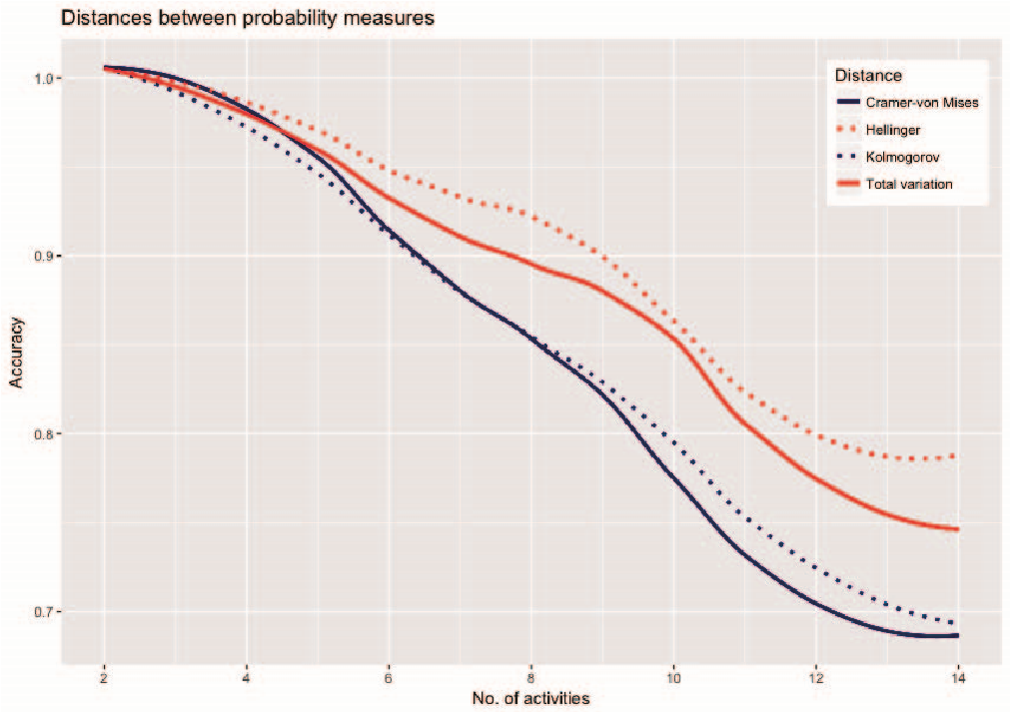
\includegraphics[scale=0.4]{Images/Picture1.png}
        \caption{Comparing the accuracy using different distance metrics between discrete empirical distributions.}
        \caption{Caption}
        \label{fig:my_label}
    \end{figure}
   
\end{frame}
\begin{frame}{Inferences}
    \begin{itemize}
        % From the above figure it is clear that
        \item Working with probability mass functions, (Hellinger and Total variation), outperforms working with cumulative distribution functions, (Cramervon Mises and Kolmogorov).
        \item Working with an L2 norm style as in the Hellinger case outperforms working with an L1 norm style as in the total variation case.\\
%Of course,
        The former is smoother and more uniform in accounting for distances among the various parts of the two input signals. 
        \item The best performance is achieved using the Hellinger distance, using the whole set of 14 activities its accuracy is about 80\%.
    \end{itemize}
\end{frame}
\section{Summary}
\begin{frame}{Summary}
    \begin{itemize}
        \item This research aimed at recognition of human activity based on probabilistic modelling of the underlying tri-axial accelerometer signal that describes the activity. 
        \item The signal is assumed to be streamed from a wearable device. 
        \item Our approach is based on representing the time series as a probability distribution, which loses the temporal succession of the streaming.
        \item Despite of this loss, the approach has shown effectiveness in the predictive performance as well as computationally.
        \item This can be attributed in part to the stationarity of the underlying time series as well as to a hypothesized short-term correlations in the given studied activities.
        \item These claims need to be verified using more datasets as well as more thorough investigation of the time series.
    \end{itemize}
\end{frame}
\begin{frame}{Summary}
    \begin{itemize}
        \item For each activity, a set of samples from the training set are chosen at random to act as templates of the activity, we called them ‘support samples’. Then, at test/operation time a new test sample is then compared %(using their representations as probability distributions)
        against each template set of each activity to decide its activity membership.
        \item The comparison is based on some typical dissimilarity metrics.
        \item It turned out that the Hellinger distance gives the best stable performance.
    \end{itemize}
\end{frame}
\begin{frame}{Prospective future work}
    \begin{itemize}
        \item The future research can investigate more diverse methods within the same paradigm of using probability distributions as representations of the signals along with multitude of distance metrics. It may also experiment with other modes of sensory data, in particular, the gyroscope.
    \end{itemize}
\end{frame}
\begin{frame}
    \centering  \Huge
    \emph{ Thank You}\\
    \vspace{2cm}
    \large
    Vibhavasu Pasumarti\\
    EP20BTECH11015

\end{frame}

\end{document}
